\documentclass[twoside]{book}

% Packages required by doxygen
\usepackage{fixltx2e}
\usepackage{calc}
\usepackage{doxygen}
\usepackage[export]{adjustbox} % also loads graphicx
\usepackage{graphicx}
\usepackage[utf8]{inputenc}
\usepackage{makeidx}
\usepackage{multicol}
\usepackage{multirow}
\PassOptionsToPackage{warn}{textcomp}
\usepackage{textcomp}
\usepackage[nointegrals]{wasysym}
\usepackage[table]{xcolor}

% Font selection
\usepackage[T1]{fontenc}
\usepackage[scaled=.90]{helvet}
\usepackage{courier}
\usepackage{amssymb}
\usepackage{sectsty}
\renewcommand{\familydefault}{\sfdefault}
\allsectionsfont{%
  \fontseries{bc}\selectfont%
  \color{darkgray}%
}
\renewcommand{\DoxyLabelFont}{%
  \fontseries{bc}\selectfont%
  \color{darkgray}%
}
\newcommand{\+}{\discretionary{\mbox{\scriptsize$\hookleftarrow$}}{}{}}

% Page & text layout
\usepackage{geometry}
\geometry{%
  a4paper,%
  top=2.5cm,%
  bottom=2.5cm,%
  left=2.5cm,%
  right=2.5cm%
}
\tolerance=750
\hfuzz=15pt
\hbadness=750
\setlength{\emergencystretch}{15pt}
\setlength{\parindent}{0cm}
\setlength{\parskip}{3ex plus 2ex minus 2ex}
\makeatletter
\renewcommand{\paragraph}{%
  \@startsection{paragraph}{4}{0ex}{-1.0ex}{1.0ex}{%
    \normalfont\normalsize\bfseries\SS@parafont%
  }%
}
\renewcommand{\subparagraph}{%
  \@startsection{subparagraph}{5}{0ex}{-1.0ex}{1.0ex}{%
    \normalfont\normalsize\bfseries\SS@subparafont%
  }%
}
\makeatother

% Headers & footers
\usepackage{fancyhdr}
\pagestyle{fancyplain}
\fancyhead[LE]{\fancyplain{}{\bfseries\thepage}}
\fancyhead[CE]{\fancyplain{}{}}
\fancyhead[RE]{\fancyplain{}{\bfseries\leftmark}}
\fancyhead[LO]{\fancyplain{}{\bfseries\rightmark}}
\fancyhead[CO]{\fancyplain{}{}}
\fancyhead[RO]{\fancyplain{}{\bfseries\thepage}}
\fancyfoot[LE]{\fancyplain{}{}}
\fancyfoot[CE]{\fancyplain{}{}}
\fancyfoot[RE]{\fancyplain{}{\bfseries\scriptsize Generated by Doxygen }}
\fancyfoot[LO]{\fancyplain{}{\bfseries\scriptsize Generated by Doxygen }}
\fancyfoot[CO]{\fancyplain{}{}}
\fancyfoot[RO]{\fancyplain{}{}}
\renewcommand{\footrulewidth}{0.4pt}
\renewcommand{\chaptermark}[1]{%
  \markboth{#1}{}%
}
\renewcommand{\sectionmark}[1]{%
  \markright{\thesection\ #1}%
}

% Indices & bibliography
\usepackage{natbib}
\usepackage[titles]{tocloft}
\setcounter{tocdepth}{3}
\setcounter{secnumdepth}{5}
\makeindex

% Hyperlinks (required, but should be loaded last)
\usepackage{ifpdf}
\ifpdf
  \usepackage[pdftex,pagebackref=true]{hyperref}
\else
  \usepackage[ps2pdf,pagebackref=true]{hyperref}
\fi
\hypersetup{%
  colorlinks=true,%
  linkcolor=blue,%
  citecolor=blue,%
  unicode%
}

% Custom commands
\newcommand{\clearemptydoublepage}{%
  \newpage{\pagestyle{empty}\cleardoublepage}%
}

\usepackage{caption}
\captionsetup{labelsep=space,justification=centering,font={bf},singlelinecheck=off,skip=4pt,position=top}

%===== C O N T E N T S =====

\begin{document}

% Titlepage & ToC
\hypersetup{pageanchor=false,
             bookmarksnumbered=true,
             pdfencoding=unicode
            }
\pagenumbering{roman}
\begin{titlepage}
\vspace*{7cm}
\begin{center}%
{\Large Genetics \\[1ex]\large 1 }\\
\vspace*{1cm}
{\large Generated by Doxygen 1.8.11}\\
\end{center}
\end{titlepage}
\clearemptydoublepage
\tableofcontents
\clearemptydoublepage
\pagenumbering{arabic}
\hypersetup{pageanchor=true}

%--- Begin generated contents ---
\chapter{Hierarchical Index}
\section{Class Hierarchy}
This inheritance list is sorted roughly, but not completely, alphabetically\+:\begin{DoxyCompactList}
\item \contentsline{section}{Allele}{\pageref{class_allele}}{}
\item \contentsline{section}{Coleman\+X\+M\+L\+Parser}{\pageref{class_coleman_x_m_l_parser}}{}
\item \contentsline{section}{Gene}{\pageref{class_gene}}{}
\item \contentsline{section}{Genetics\+Sim\+Data\+Parser}{\pageref{class_genetics_sim_data_parser}}{}
\item \contentsline{section}{I\+File\+Parser}{\pageref{struct_i_file_parser}}{}
\item \contentsline{section}{I\+Observable}{\pageref{class_i_observable}}{}
\begin{DoxyCompactList}
\item \contentsline{section}{Love\+Chamber}{\pageref{class_love_chamber}}{}
\end{DoxyCompactList}
\item \contentsline{section}{I\+Observer$<$ T $>$}{\pageref{struct_i_observer}}{}
\begin{DoxyCompactList}
\item \contentsline{section}{Stat\+Counter}{\pageref{class_stat_counter}}{}
\end{DoxyCompactList}
\item \contentsline{section}{I\+Observer$<$ Organism $>$}{\pageref{struct_i_observer}}{}
\begin{DoxyCompactList}
\item \contentsline{section}{Stat\+Counter}{\pageref{class_stat_counter}}{}
\end{DoxyCompactList}
\item \contentsline{section}{Observable$<$ T $>$}{\pageref{class_observable}}{}
\item \contentsline{section}{Observable$<$ Organism $>$}{\pageref{class_observable}}{}
\begin{DoxyCompactList}
\item \contentsline{section}{Love\+Chamber}{\pageref{class_love_chamber}}{}
\end{DoxyCompactList}
\item \contentsline{section}{Organism}{\pageref{class_organism}}{}
\item \contentsline{section}{Simulation}{\pageref{class_simulation}}{}
\end{DoxyCompactList}

\chapter{Class Index}
\section{Class List}
Here are the classes, structs, unions and interfaces with brief descriptions\+:\begin{DoxyCompactList}
\item\contentsline{section}{\hyperlink{class_allele}{Allele} \\*Models the alleles of a \hyperlink{class_gene}{Gene} }{\pageref{class_allele}}{}
\item\contentsline{section}{\hyperlink{class_coleman_x_m_l_parser}{Coleman\+X\+M\+L\+Parser} \\*Wraps behavior of \hyperlink{class_genetics_sim_data_parser}{Genetics\+Sim\+Data\+Parser} }{\pageref{class_coleman_x_m_l_parser}}{}
\item\contentsline{section}{\hyperlink{class_empty_container_exception}{Empty\+Container\+Exception} \\*Exception for empty containers }{\pageref{class_empty_container_exception}}{}
\item\contentsline{section}{\hyperlink{class_gene}{Gene} \\*Handles pairs of \hyperlink{class_allele}{Allele} }{\pageref{class_gene}}{}
\item\contentsline{section}{\hyperlink{class_genetics_sim_data_parser}{Genetics\+Sim\+Data\+Parser} }{\pageref{class_genetics_sim_data_parser}}{}
\item\contentsline{section}{\hyperlink{struct_i_observer}{I\+Observer$<$ T $>$} \\*The \hyperlink{struct_i_observer}{I\+Observer} class is an interface for observers }{\pageref{struct_i_observer}}{}
\item\contentsline{section}{\hyperlink{class_love_chamber}{Love\+Chamber} \\*Handles mating between Organisms }{\pageref{class_love_chamber}}{}
\item\contentsline{section}{\hyperlink{class_malformed_file_exception}{Malformed\+File\+Exception} \\*Exception for malformed files }{\pageref{class_malformed_file_exception}}{}
\item\contentsline{section}{\hyperlink{class_observable}{Observable$<$ T $>$} \\*The \hyperlink{class_observable}{Observable} class is an interface for observable objects }{\pageref{class_observable}}{}
\item\contentsline{section}{\hyperlink{class_organism}{Organism} \\*Living thing }{\pageref{class_organism}}{}
\item\contentsline{section}{\hyperlink{class_simulation}{Simulation} \\*Handles the main thread of execution for the genetic simulation }{\pageref{class_simulation}}{}
\item\contentsline{section}{\hyperlink{class_stat_counter}{Stat\+Counter} \\*Records statistical data of Organisms }{\pageref{class_stat_counter}}{}
\end{DoxyCompactList}

\chapter{Class Documentation}
\hypertarget{class_allele}{}\section{Allele Class Reference}
\label{class_allele}\index{Allele@{Allele}}


The \hyperlink{class_allele}{Allele} class models the alleles of a \hyperlink{class_gene}{Gene}.  




{\ttfamily \#include $<$Allele.\+h$>$}

\subsection*{Public Member Functions}
\begin{DoxyCompactItemize}
\item 
\hyperlink{class_allele_a22adf689d715473f8a14fdc2ac80e167}{Allele} (char symbol, const std\+::string \&description)
\begin{DoxyCompactList}\small\item\em Constructs an \hyperlink{class_allele}{Allele} object. \end{DoxyCompactList}\item 
bool \hyperlink{class_allele_a6096e43a00dfc291544abd97b4a82c06}{is\+Dominant} () const 
\item 
char \hyperlink{class_allele_afc738a4cfcc3e69e07baf2e196570c0a}{get\+Symbol} () const 
\item 
std\+::string \hyperlink{class_allele_a332bec024b1be3eff4ba984320aed490}{get\+Description} () const 
\end{DoxyCompactItemize}


\subsection{Detailed Description}
The \hyperlink{class_allele}{Allele} class models the alleles of a \hyperlink{class_gene}{Gene}. 

This immutable representation of an allele holds information regarding symbols (e.\+g. T or t), description of the allele (e.\+g. tall), and whether the allele is dominant or not. It is an essential part of the \hyperlink{class_gene}{Gene} class. \begin{DoxySeeAlso}{See also}
\hyperlink{class_gene}{Gene} 
\end{DoxySeeAlso}


\subsection{Constructor \& Destructor Documentation}
\index{Allele@{Allele}!Allele@{Allele}}
\index{Allele@{Allele}!Allele@{Allele}}
\subsubsection[{\texorpdfstring{Allele(char symbol, const std\+::string \&description)}{Allele(char symbol, const std::string &description)}}]{\setlength{\rightskip}{0pt plus 5cm}Allele\+::\+Allele (
\begin{DoxyParamCaption}
\item[{char}]{symbol, }
\item[{const std\+::string \&}]{description}
\end{DoxyParamCaption}
)}\hypertarget{class_allele_a22adf689d715473f8a14fdc2ac80e167}{}\label{class_allele_a22adf689d715473f8a14fdc2ac80e167}


Constructs an \hyperlink{class_allele}{Allele} object. 


\begin{DoxyParams}{Parameters}
{\em symbol} & The symbol for the allele \\
\hline
{\em description} & What the allele represents \\
\hline
\end{DoxyParams}


\subsection{Member Function Documentation}
\index{Allele@{Allele}!get\+Description@{get\+Description}}
\index{get\+Description@{get\+Description}!Allele@{Allele}}
\subsubsection[{\texorpdfstring{get\+Description() const }{getDescription() const }}]{\setlength{\rightskip}{0pt plus 5cm}std\+::string Allele\+::get\+Description (
\begin{DoxyParamCaption}
{}
\end{DoxyParamCaption}
) const\hspace{0.3cm}{\ttfamily [inline]}}\hypertarget{class_allele_a332bec024b1be3eff4ba984320aed490}{}\label{class_allele_a332bec024b1be3eff4ba984320aed490}
\begin{DoxyReturn}{Returns}
The description of the allele (e.\+g. \char`\"{}tall\char`\"{} or \char`\"{}short\char`\"{}) 
\end{DoxyReturn}
\index{Allele@{Allele}!get\+Symbol@{get\+Symbol}}
\index{get\+Symbol@{get\+Symbol}!Allele@{Allele}}
\subsubsection[{\texorpdfstring{get\+Symbol() const }{getSymbol() const }}]{\setlength{\rightskip}{0pt plus 5cm}char Allele\+::get\+Symbol (
\begin{DoxyParamCaption}
{}
\end{DoxyParamCaption}
) const\hspace{0.3cm}{\ttfamily [inline]}}\hypertarget{class_allele_afc738a4cfcc3e69e07baf2e196570c0a}{}\label{class_allele_afc738a4cfcc3e69e07baf2e196570c0a}
\begin{DoxyReturn}{Returns}
The symbol of the allele (e.\+g. \textquotesingle{}T\textquotesingle{} or \textquotesingle{}t\textquotesingle{}) 
\end{DoxyReturn}
\index{Allele@{Allele}!is\+Dominant@{is\+Dominant}}
\index{is\+Dominant@{is\+Dominant}!Allele@{Allele}}
\subsubsection[{\texorpdfstring{is\+Dominant() const }{isDominant() const }}]{\setlength{\rightskip}{0pt plus 5cm}bool Allele\+::is\+Dominant (
\begin{DoxyParamCaption}
{}
\end{DoxyParamCaption}
) const\hspace{0.3cm}{\ttfamily [inline]}}\hypertarget{class_allele_a6096e43a00dfc291544abd97b4a82c06}{}\label{class_allele_a6096e43a00dfc291544abd97b4a82c06}
\begin{DoxyReturn}{Returns}
True if the allele is dominant or false if it is recessive 
\end{DoxyReturn}


The documentation for this class was generated from the following files\+:\begin{DoxyCompactItemize}
\item 
Genetics/Allele.\+h\item 
Genetics/Allele.\+cpp\end{DoxyCompactItemize}

\hypertarget{class_coleman_x_m_l_parser}{}\section{Coleman\+X\+M\+L\+Parser Class Reference}
\label{class_coleman_x_m_l_parser}\index{Coleman\+X\+M\+L\+Parser@{Coleman\+X\+M\+L\+Parser}}


The \hyperlink{class_coleman_x_m_l_parser}{Coleman\+X\+M\+L\+Parser} class wraps behavior of \hyperlink{class_genetics_sim_data_parser}{Genetics\+Sim\+Data\+Parser}.  




{\ttfamily \#include $<$Coleman\+X\+M\+L\+Parser.\+h$>$}

\subsection*{Public Member Functions}
\begin{DoxyCompactItemize}
\item 
\hypertarget{class_coleman_x_m_l_parser_a8eda751b3cb0b3f94add5a24fddacbc1}{}{\bfseries Coleman\+X\+M\+L\+Parser} (const string \&filename)\label{class_coleman_x_m_l_parser_a8eda751b3cb0b3f94add5a24fddacbc1}

\item 
void \hyperlink{class_coleman_x_m_l_parser_ae168a5ae05ee145556a7b1f612fde3ea}{parse\+File} (std\+::vector$<$ \hyperlink{class_organism}{Organism} $>$ \&organisms)
\begin{DoxyCompactList}\small\item\em Reads organism data from a file into a vector of organisms. \end{DoxyCompactList}\end{DoxyCompactItemize}


\subsection{Detailed Description}
The \hyperlink{class_coleman_x_m_l_parser}{Coleman\+X\+M\+L\+Parser} class wraps behavior of \hyperlink{class_genetics_sim_data_parser}{Genetics\+Sim\+Data\+Parser}. 

This class acts as a wrapper around Dr. Coleman\textquotesingle{}s \hyperlink{class_genetics_sim_data_parser}{Genetics\+Sim\+Data\+Parser} class. It takes a filename which should contain organism data and then stores that data in a supplied container. \begin{DoxySeeAlso}{See also}
\hyperlink{class_genetics_sim_data_parser}{Genetics\+Sim\+Data\+Parser} 
\end{DoxySeeAlso}


\subsection{Member Function Documentation}
\hypertarget{class_coleman_x_m_l_parser_ae168a5ae05ee145556a7b1f612fde3ea}{}\index{Coleman\+X\+M\+L\+Parser@{Coleman\+X\+M\+L\+Parser}!parse\+File@{parse\+File}}
\index{parse\+File@{parse\+File}!Coleman\+X\+M\+L\+Parser@{Coleman\+X\+M\+L\+Parser}}
\subsubsection[{parse\+File}]{\setlength{\rightskip}{0pt plus 5cm}void Coleman\+X\+M\+L\+Parser\+::parse\+File (
\begin{DoxyParamCaption}
\item[{std\+::vector$<$ {\bf Organism} $>$ \&}]{organisms}
\end{DoxyParamCaption}
)}\label{class_coleman_x_m_l_parser_ae168a5ae05ee145556a7b1f612fde3ea}


Reads organism data from a file into a vector of organisms. 


\begin{DoxyParams}{Parameters}
{\em organisms} & The vector to store the organisms in \\
\hline
{\em expected\+Count} & The expected organism count in the data file \\
\hline
\end{DoxyParams}
\begin{DoxySeeAlso}{See also}
\hyperlink{class_organism}{Organism} 
\end{DoxySeeAlso}


The documentation for this class was generated from the following files\+:\begin{DoxyCompactItemize}
\item 
Genetics/Coleman\+X\+M\+L\+Parser.\+h\item 
Genetics/Coleman\+X\+M\+L\+Parser.\+cpp\end{DoxyCompactItemize}

\hypertarget{class_gene}{}\section{Gene Class Reference}
\label{class_gene}\index{Gene@{Gene}}


The \hyperlink{class_gene}{Gene} class handles pairs of \hyperlink{class_allele}{Allele}.  




{\ttfamily \#include $<$Gene-\/a\+Computer.\+h$>$}

\subsection*{Public Member Functions}
\begin{DoxyCompactItemize}
\item 
\hyperlink{class_gene_a3e8f531d014dd6aa2cfb25c7fed5ae5d}{Gene} (const \hyperlink{class_allele}{Allele} \&a1, const \hyperlink{class_allele}{Allele} \&a2, const std\+::string \&desc)
\begin{DoxyCompactList}\small\item\em Constructs a \hyperlink{class_gene}{Gene} object. \end{DoxyCompactList}\item 
\hyperlink{class_allele}{Allele} \hyperlink{class_gene_a7b631b7a53729db7523430049c89e463}{get\+Random\+Allele} () const 
\begin{DoxyCompactList}\small\item\em Picks a random \hyperlink{class_allele}{Allele} from the pair and returns it. \end{DoxyCompactList}\item 
\hyperlink{class_allele}{Allele} \hyperlink{class_gene_a935e5f290b1e66b970ed8b52a97b1ae9}{first} () const 
\item 
\hyperlink{class_allele}{Allele} \hyperlink{class_gene_a7c744b5c6e8d305c47c1563cc0e2acc8}{second} () const 
\item 
std\+::string \hyperlink{class_gene_a3d5569b6329c23acf791ce310735fc5d}{to\+String} () const 
\item 
\hyperlink{class_gene_a3e8f531d014dd6aa2cfb25c7fed5ae5d}{Gene} (const \hyperlink{class_allele}{Allele} \&a1, const \hyperlink{class_allele}{Allele} \&a2, const std\+::string \&desc)
\begin{DoxyCompactList}\small\item\em Constructs a \hyperlink{class_gene}{Gene} object. \end{DoxyCompactList}\item 
\hyperlink{class_allele}{Allele} \hyperlink{class_gene_a7b631b7a53729db7523430049c89e463}{get\+Random\+Allele} () const 
\begin{DoxyCompactList}\small\item\em Picks a random \hyperlink{class_allele}{Allele} from the pair and returns it. \end{DoxyCompactList}\item 
\hyperlink{class_allele}{Allele} \hyperlink{class_gene_a935e5f290b1e66b970ed8b52a97b1ae9}{first} () const 
\item 
\hyperlink{class_allele}{Allele} \hyperlink{class_gene_a7c744b5c6e8d305c47c1563cc0e2acc8}{second} () const 
\item 
std\+::string {\bfseries get\+Description} () const \hypertarget{class_gene_ad25e29f23ead79aa820a6df83ce37f21}{}\label{class_gene_ad25e29f23ead79aa820a6df83ce37f21}

\item 
std\+::string \hyperlink{class_gene_a97e77e08f0ade2ebe413aab5a2160007}{get\+Phenotype} () const 
\item 
std\+::string \hyperlink{class_gene_a9b88c16c2408458ca43a82cdc4d5cbe3}{get\+Zygosity} () const 
\item 
std\+::string \hyperlink{class_gene_ab4b2614b4481851fcbd61860c464406f}{get\+Alleles\+String} () const 
\item 
std\+::string \hyperlink{class_gene_a3d5569b6329c23acf791ce310735fc5d}{to\+String} () const 
\end{DoxyCompactItemize}


\subsection{Detailed Description}
The \hyperlink{class_gene}{Gene} class handles pairs of \hyperlink{class_allele}{Allele}. 

\hyperlink{class_gene}{Gene} holds a pair of Alleles that can be any combination of dominant or recessive. It is immutable and allows the random retrieval of copies of either of the stored Alleles. \begin{DoxySeeAlso}{See also}
\hyperlink{class_allele}{Allele} 
\end{DoxySeeAlso}


\subsection{Constructor \& Destructor Documentation}
\index{Gene@{Gene}!Gene@{Gene}}
\index{Gene@{Gene}!Gene@{Gene}}
\subsubsection[{\texorpdfstring{Gene(const Allele \&a1, const Allele \&a2, const std\+::string \&desc)}{Gene(const Allele &a1, const Allele &a2, const std::string &desc)}}]{\setlength{\rightskip}{0pt plus 5cm}Gene\+::\+Gene (
\begin{DoxyParamCaption}
\item[{const {\bf Allele} \&}]{a1, }
\item[{const {\bf Allele} \&}]{a2, }
\item[{const std\+::string \&}]{desc}
\end{DoxyParamCaption}
)}\hypertarget{class_gene_a3e8f531d014dd6aa2cfb25c7fed5ae5d}{}\label{class_gene_a3e8f531d014dd6aa2cfb25c7fed5ae5d}


Constructs a \hyperlink{class_gene}{Gene} object. 


\begin{DoxyParams}{Parameters}
{\em a1} & One allele to be part of the gene \\
\hline
{\em a2} & One allele to be part of the gene \\
\hline
{\em desc} & The description of the gene trait \\
\hline
\end{DoxyParams}
\index{Gene@{Gene}!Gene@{Gene}}
\index{Gene@{Gene}!Gene@{Gene}}
\subsubsection[{\texorpdfstring{Gene(const Allele \&a1, const Allele \&a2, const std\+::string \&desc)}{Gene(const Allele &a1, const Allele &a2, const std::string &desc)}}]{\setlength{\rightskip}{0pt plus 5cm}Gene\+::\+Gene (
\begin{DoxyParamCaption}
\item[{const {\bf Allele} \&}]{a1, }
\item[{const {\bf Allele} \&}]{a2, }
\item[{const std\+::string \&}]{desc}
\end{DoxyParamCaption}
)}\hypertarget{class_gene_a3e8f531d014dd6aa2cfb25c7fed5ae5d}{}\label{class_gene_a3e8f531d014dd6aa2cfb25c7fed5ae5d}


Constructs a \hyperlink{class_gene}{Gene} object. 


\begin{DoxyParams}{Parameters}
{\em a1} & One allele to be part of the gene \\
\hline
{\em a2} & One allele to be part of the gene \\
\hline
{\em desc} & The description of the gene trait \\
\hline
\end{DoxyParams}


\subsection{Member Function Documentation}
\index{Gene@{Gene}!first@{first}}
\index{first@{first}!Gene@{Gene}}
\subsubsection[{\texorpdfstring{first() const }{first() const }}]{\setlength{\rightskip}{0pt plus 5cm}{\bf Allele} Gene\+::first (
\begin{DoxyParamCaption}
{}
\end{DoxyParamCaption}
) const\hspace{0.3cm}{\ttfamily [inline]}}\hypertarget{class_gene_a935e5f290b1e66b970ed8b52a97b1ae9}{}\label{class_gene_a935e5f290b1e66b970ed8b52a97b1ae9}
\begin{DoxyReturn}{Returns}
The first of two alleles 
\end{DoxyReturn}
\index{Gene@{Gene}!first@{first}}
\index{first@{first}!Gene@{Gene}}
\subsubsection[{\texorpdfstring{first() const }{first() const }}]{\setlength{\rightskip}{0pt plus 5cm}{\bf Allele} Gene\+::first (
\begin{DoxyParamCaption}
{}
\end{DoxyParamCaption}
) const\hspace{0.3cm}{\ttfamily [inline]}}\hypertarget{class_gene_a935e5f290b1e66b970ed8b52a97b1ae9}{}\label{class_gene_a935e5f290b1e66b970ed8b52a97b1ae9}
\begin{DoxyReturn}{Returns}
The first of two alleles 
\end{DoxyReturn}
\index{Gene@{Gene}!get\+Alleles\+String@{get\+Alleles\+String}}
\index{get\+Alleles\+String@{get\+Alleles\+String}!Gene@{Gene}}
\subsubsection[{\texorpdfstring{get\+Alleles\+String() const }{getAllelesString() const }}]{\setlength{\rightskip}{0pt plus 5cm}std\+::string Gene\+::get\+Alleles\+String (
\begin{DoxyParamCaption}
{}
\end{DoxyParamCaption}
) const}\hypertarget{class_gene_ab4b2614b4481851fcbd61860c464406f}{}\label{class_gene_ab4b2614b4481851fcbd61860c464406f}
\begin{DoxyReturn}{Returns}
The allele pair of the gene as a string 
\end{DoxyReturn}
\index{Gene@{Gene}!get\+Phenotype@{get\+Phenotype}}
\index{get\+Phenotype@{get\+Phenotype}!Gene@{Gene}}
\subsubsection[{\texorpdfstring{get\+Phenotype() const }{getPhenotype() const }}]{\setlength{\rightskip}{0pt plus 5cm}std\+::string Gene\+::get\+Phenotype (
\begin{DoxyParamCaption}
{}
\end{DoxyParamCaption}
) const}\hypertarget{class_gene_a97e77e08f0ade2ebe413aab5a2160007}{}\label{class_gene_a97e77e08f0ade2ebe413aab5a2160007}
\begin{DoxyReturn}{Returns}
The phenotype of the gene 
\end{DoxyReturn}
\index{Gene@{Gene}!get\+Random\+Allele@{get\+Random\+Allele}}
\index{get\+Random\+Allele@{get\+Random\+Allele}!Gene@{Gene}}
\subsubsection[{\texorpdfstring{get\+Random\+Allele() const }{getRandomAllele() const }}]{\setlength{\rightskip}{0pt plus 5cm}{\bf Allele} Gene\+::get\+Random\+Allele (
\begin{DoxyParamCaption}
{}
\end{DoxyParamCaption}
) const}\hypertarget{class_gene_a7b631b7a53729db7523430049c89e463}{}\label{class_gene_a7b631b7a53729db7523430049c89e463}


Picks a random \hyperlink{class_allele}{Allele} from the pair and returns it. 

\begin{DoxyReturn}{Returns}
An \hyperlink{class_allele}{Allele} from the pair 
\end{DoxyReturn}
\index{Gene@{Gene}!get\+Random\+Allele@{get\+Random\+Allele}}
\index{get\+Random\+Allele@{get\+Random\+Allele}!Gene@{Gene}}
\subsubsection[{\texorpdfstring{get\+Random\+Allele() const }{getRandomAllele() const }}]{\setlength{\rightskip}{0pt plus 5cm}{\bf Allele} Gene\+::get\+Random\+Allele (
\begin{DoxyParamCaption}
{}
\end{DoxyParamCaption}
) const}\hypertarget{class_gene_a7b631b7a53729db7523430049c89e463}{}\label{class_gene_a7b631b7a53729db7523430049c89e463}


Picks a random \hyperlink{class_allele}{Allele} from the pair and returns it. 

\begin{DoxyReturn}{Returns}
An \hyperlink{class_allele}{Allele} from the pair 
\end{DoxyReturn}
\index{Gene@{Gene}!get\+Zygosity@{get\+Zygosity}}
\index{get\+Zygosity@{get\+Zygosity}!Gene@{Gene}}
\subsubsection[{\texorpdfstring{get\+Zygosity() const }{getZygosity() const }}]{\setlength{\rightskip}{0pt plus 5cm}std\+::string Gene\+::get\+Zygosity (
\begin{DoxyParamCaption}
{}
\end{DoxyParamCaption}
) const}\hypertarget{class_gene_a9b88c16c2408458ca43a82cdc4d5cbe3}{}\label{class_gene_a9b88c16c2408458ca43a82cdc4d5cbe3}
\begin{DoxyReturn}{Returns}
The zygosity of the gene (i.\+e. heterozygous, etc) 
\end{DoxyReturn}
\index{Gene@{Gene}!second@{second}}
\index{second@{second}!Gene@{Gene}}
\subsubsection[{\texorpdfstring{second() const }{second() const }}]{\setlength{\rightskip}{0pt plus 5cm}{\bf Allele} Gene\+::second (
\begin{DoxyParamCaption}
{}
\end{DoxyParamCaption}
) const\hspace{0.3cm}{\ttfamily [inline]}}\hypertarget{class_gene_a7c744b5c6e8d305c47c1563cc0e2acc8}{}\label{class_gene_a7c744b5c6e8d305c47c1563cc0e2acc8}
\begin{DoxyReturn}{Returns}
The second of two alleles 
\end{DoxyReturn}
\index{Gene@{Gene}!second@{second}}
\index{second@{second}!Gene@{Gene}}
\subsubsection[{\texorpdfstring{second() const }{second() const }}]{\setlength{\rightskip}{0pt plus 5cm}{\bf Allele} Gene\+::second (
\begin{DoxyParamCaption}
{}
\end{DoxyParamCaption}
) const\hspace{0.3cm}{\ttfamily [inline]}}\hypertarget{class_gene_a7c744b5c6e8d305c47c1563cc0e2acc8}{}\label{class_gene_a7c744b5c6e8d305c47c1563cc0e2acc8}
\begin{DoxyReturn}{Returns}
The second of two alleles 
\end{DoxyReturn}
\index{Gene@{Gene}!to\+String@{to\+String}}
\index{to\+String@{to\+String}!Gene@{Gene}}
\subsubsection[{\texorpdfstring{to\+String() const }{toString() const }}]{\setlength{\rightskip}{0pt plus 5cm}std\+::string Gene\+::to\+String (
\begin{DoxyParamCaption}
{}
\end{DoxyParamCaption}
) const}\hypertarget{class_gene_a3d5569b6329c23acf791ce310735fc5d}{}\label{class_gene_a3d5569b6329c23acf791ce310735fc5d}
\begin{DoxyReturn}{Returns}
The allele pair of the gene as a string 
\end{DoxyReturn}
\index{Gene@{Gene}!to\+String@{to\+String}}
\index{to\+String@{to\+String}!Gene@{Gene}}
\subsubsection[{\texorpdfstring{to\+String() const }{toString() const }}]{\setlength{\rightskip}{0pt plus 5cm}std\+::string Gene\+::to\+String (
\begin{DoxyParamCaption}
{}
\end{DoxyParamCaption}
) const}\hypertarget{class_gene_a3d5569b6329c23acf791ce310735fc5d}{}\label{class_gene_a3d5569b6329c23acf791ce310735fc5d}
\begin{DoxyReturn}{Returns}
The fully qualified description of the gene 
\end{DoxyReturn}


The documentation for this class was generated from the following files\+:\begin{DoxyCompactItemize}
\item 
Genetics/Gene-\/a\+Computer.\+h\item 
Genetics/Gene.\+h\item 
Genetics/Gene-\/a\+Computer.\+cpp\item 
Genetics/Gene.\+cpp\end{DoxyCompactItemize}

\hypertarget{class_genetics_sim_data_parser}{}\section{Genetics\+Sim\+Data\+Parser Class Reference}
\label{class_genetics_sim_data_parser}\index{Genetics\+Sim\+Data\+Parser@{Genetics\+Sim\+Data\+Parser}}
\subsection*{Public Member Functions}
\begin{DoxyCompactItemize}
\item 
\hypertarget{class_genetics_sim_data_parser_a1115728ef64adaca0882855775a03fde}{}{\bfseries Genetics\+Sim\+Data\+Parser} (char $\ast$file\+Name)\label{class_genetics_sim_data_parser_a1115728ef64adaca0882855775a03fde}

\item 
\hypertarget{class_genetics_sim_data_parser_af5d625aef87b4e893d755ef8ba284a89}{}int {\bfseries get\+Gene\+Count} ()\label{class_genetics_sim_data_parser_af5d625aef87b4e893d755ef8ba284a89}

\item 
\hypertarget{class_genetics_sim_data_parser_a50adc731a54bda327aa49d5e173abbe3}{}char $\ast$ {\bfseries get\+Genus} ()\label{class_genetics_sim_data_parser_a50adc731a54bda327aa49d5e173abbe3}

\item 
\hypertarget{class_genetics_sim_data_parser_ac13e07486db1c65aed87a0b6249c4e51}{}char $\ast$ {\bfseries get\+Species} ()\label{class_genetics_sim_data_parser_ac13e07486db1c65aed87a0b6249c4e51}

\item 
\hypertarget{class_genetics_sim_data_parser_a1541715a692c012f0f3fbe8a997ff3fd}{}char $\ast$ {\bfseries get\+Scientific\+Name} ()\label{class_genetics_sim_data_parser_a1541715a692c012f0f3fbe8a997ff3fd}

\item 
\hypertarget{class_genetics_sim_data_parser_a23a7f0ae3ce3230962800d8cb81bdd61}{}char $\ast$ {\bfseries get\+Common\+Name} ()\label{class_genetics_sim_data_parser_a23a7f0ae3ce3230962800d8cb81bdd61}

\item 
\hypertarget{class_genetics_sim_data_parser_a68e7b81cf5b921c3483e6aa0bad461ec}{}bool {\bfseries get\+Parent\+Genotype} (char $\ast$genotype)\label{class_genetics_sim_data_parser_a68e7b81cf5b921c3483e6aa0bad461ec}

\item 
\hypertarget{class_genetics_sim_data_parser_a6b20d5399593182ea3cedf189c67bc5a}{}bool {\bfseries get\+Gene\+Data} (char $\ast$trait, char $\ast$dom\+Desc, char $\ast$dom\+Symbol, char $\ast$rec\+Desc, char $\ast$rec\+Symbol)\label{class_genetics_sim_data_parser_a6b20d5399593182ea3cedf189c67bc5a}

\end{DoxyCompactItemize}


The documentation for this class was generated from the following files\+:\begin{DoxyCompactItemize}
\item 
Genetics/Genetics\+Sim\+Data\+Parser.\+h\item 
Genetics/Genetics\+Sim\+Data\+Parser.\+cpp\end{DoxyCompactItemize}

\hypertarget{struct_i_observer}{}\section{I\+Observer$<$ T $>$ Struct Template Reference}
\label{struct_i_observer}\index{I\+Observer$<$ T $>$@{I\+Observer$<$ T $>$}}
Inheritance diagram for I\+Observer$<$ T $>$\+:\begin{figure}[H]
\begin{center}
\leavevmode
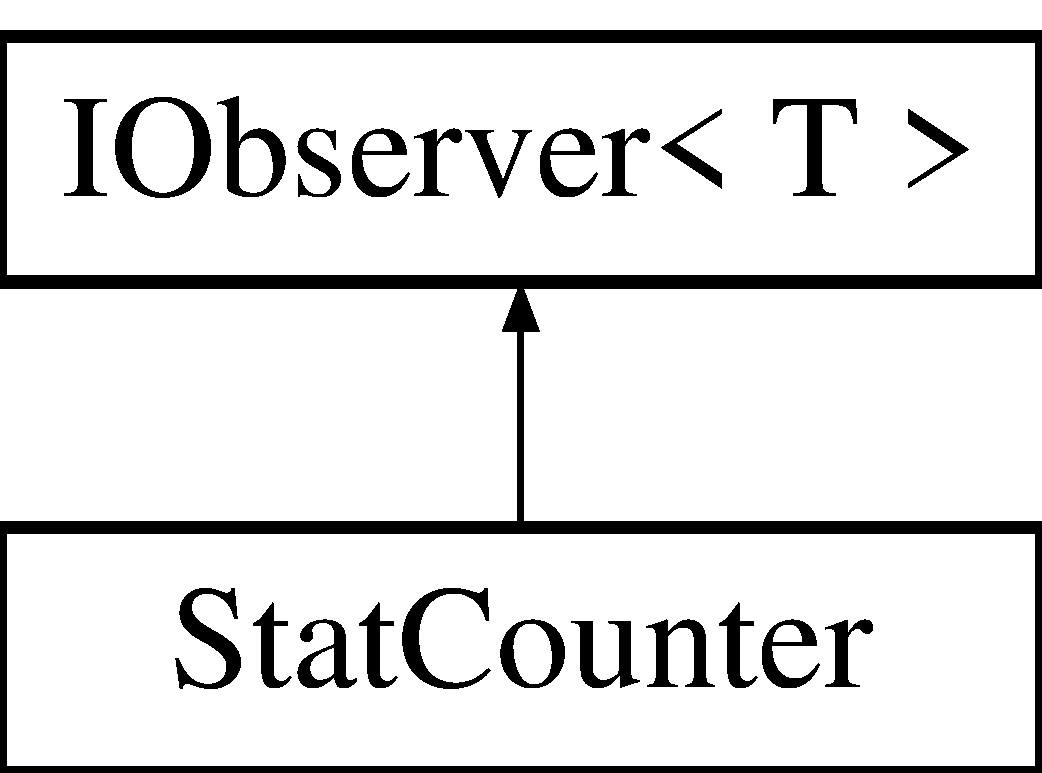
\includegraphics[height=2.000000cm]{struct_i_observer}
\end{center}
\end{figure}
\subsection*{Public Member Functions}
\begin{DoxyCompactItemize}
\item 
virtual void {\bfseries notify} (const std\+::string \&arg)=0\hypertarget{struct_i_observer_a51f5898305d0a9004e9c7126c9015a45}{}\label{struct_i_observer_a51f5898305d0a9004e9c7126c9015a45}

\item 
virtual void {\bfseries notify} (const T \&arg)=0\hypertarget{struct_i_observer_a218fcc53f11b591e002c7f3552b26a78}{}\label{struct_i_observer_a218fcc53f11b591e002c7f3552b26a78}

\end{DoxyCompactItemize}


The documentation for this struct was generated from the following files\+:\begin{DoxyCompactItemize}
\item 
Genetics/I\+Observer-\/a\+Computer.\+h\item 
Genetics/I\+Observer.\+h\end{DoxyCompactItemize}

\hypertarget{class_love_chamber}{}\section{Love\+Chamber Class Reference}
\label{class_love_chamber}\index{Love\+Chamber@{Love\+Chamber}}


The \hyperlink{class_love_chamber}{Love\+Chamber} class handles mating between Organisms.  




{\ttfamily \#include $<$Love\+Chamber.\+h$>$}

Inheritance diagram for Love\+Chamber\+:\begin{figure}[H]
\begin{center}
\leavevmode
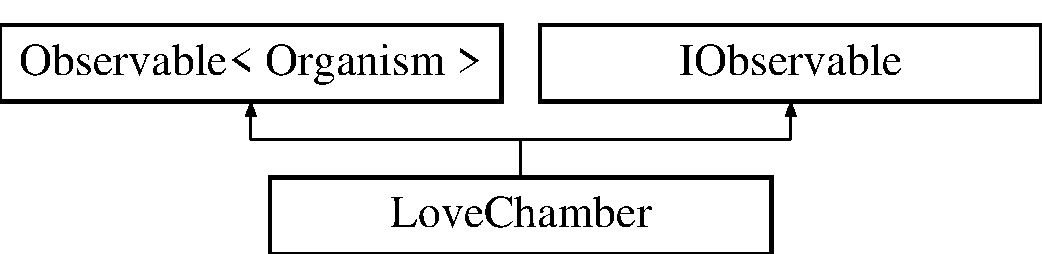
\includegraphics[height=2.000000cm]{class_love_chamber}
\end{center}
\end{figure}
\subsection*{Public Member Functions}
\begin{DoxyCompactItemize}
\item 
\hyperlink{class_love_chamber_afd8934456036b6252e0e968c26ffb04e}{Love\+Chamber} (\hyperlink{class_organism}{Organism} o1, \hyperlink{class_organism}{Organism} o2)
\begin{DoxyCompactList}\small\item\em Constructs a \hyperlink{class_love_chamber}{Love\+Chamber} capable of producing offspring. \end{DoxyCompactList}\item 
void \hyperlink{class_love_chamber_acdb1a279b4b6edfd8d38375c4faee182}{mate} ()
\begin{DoxyCompactList}\small\item\em Creates an offspring using two parent Organisms. \end{DoxyCompactList}\end{DoxyCompactItemize}
\subsection*{Additional Inherited Members}


\subsection{Detailed Description}
The \hyperlink{class_love_chamber}{Love\+Chamber} class handles mating between Organisms. 

\hyperlink{class_love_chamber}{Love\+Chamber} uses the genotype of two Organisms to perform random crosses between the individual genotypes of each parent. The resulting offspring are sent to classes that observe \hyperlink{class_love_chamber}{Love\+Chamber}. \begin{DoxySeeAlso}{See also}
\hyperlink{class_organism}{Organism}, \hyperlink{class_observable}{Observable} 
\end{DoxySeeAlso}


\subsection{Constructor \& Destructor Documentation}
\index{Love\+Chamber@{Love\+Chamber}!Love\+Chamber@{Love\+Chamber}}
\index{Love\+Chamber@{Love\+Chamber}!Love\+Chamber@{Love\+Chamber}}
\subsubsection[{\texorpdfstring{Love\+Chamber(\+Organism o1, Organism o2)}{LoveChamber(Organism o1, Organism o2)}}]{\setlength{\rightskip}{0pt plus 5cm}Love\+Chamber\+::\+Love\+Chamber (
\begin{DoxyParamCaption}
\item[{{\bf Organism}}]{o1, }
\item[{{\bf Organism}}]{o2}
\end{DoxyParamCaption}
)}\hypertarget{class_love_chamber_afd8934456036b6252e0e968c26ffb04e}{}\label{class_love_chamber_afd8934456036b6252e0e968c26ffb04e}


Constructs a \hyperlink{class_love_chamber}{Love\+Chamber} capable of producing offspring. 


\begin{DoxyParams}{Parameters}
{\em o1} & one parent of potential offspring \\
\hline
{\em o2} & one parent of potential offspring \\
\hline
\end{DoxyParams}


\subsection{Member Function Documentation}
\index{Love\+Chamber@{Love\+Chamber}!mate@{mate}}
\index{mate@{mate}!Love\+Chamber@{Love\+Chamber}}
\subsubsection[{\texorpdfstring{mate()}{mate()}}]{\setlength{\rightskip}{0pt plus 5cm}void Love\+Chamber\+::mate (
\begin{DoxyParamCaption}
{}
\end{DoxyParamCaption}
)}\hypertarget{class_love_chamber_acdb1a279b4b6edfd8d38375c4faee182}{}\label{class_love_chamber_acdb1a279b4b6edfd8d38375c4faee182}


Creates an offspring using two parent Organisms. 

Uses the genotype of both organisms to create a random, new genotype that will belong to some offspring that is then sent to all Observers 

The documentation for this class was generated from the following files\+:\begin{DoxyCompactItemize}
\item 
Genetics/Love\+Chamber.\+h\item 
Genetics/Love\+Chamber.\+cpp\end{DoxyCompactItemize}

\hypertarget{class_observable}{}\section{Observable$<$ T $>$ Class Template Reference}
\label{class_observable}\index{Observable$<$ T $>$@{Observable$<$ T $>$}}
\subsection*{Public Member Functions}
\begin{DoxyCompactItemize}
\item 
void {\bfseries add\+Observer} (\hyperlink{struct_i_observer}{I\+Observer}$<$ T $>$ \&o)\hypertarget{class_observable_a5caccd0c60c6e11843be0ee0197d34e1}{}\label{class_observable_a5caccd0c60c6e11843be0ee0197d34e1}

\item 
void {\bfseries remove\+Observer} (const \hyperlink{struct_i_observer}{I\+Observer}$<$ T $>$ \&o)\hypertarget{class_observable_a88784c910caefa3a830025209d71adb3}{}\label{class_observable_a88784c910caefa3a830025209d71adb3}

\item 
void {\bfseries notify\+All} (const T \&arg)\hypertarget{class_observable_a2f2f224a73edbb6d42f6534ba0d28602}{}\label{class_observable_a2f2f224a73edbb6d42f6534ba0d28602}

\end{DoxyCompactItemize}
\subsection*{Protected Attributes}
\begin{DoxyCompactItemize}
\item 
std\+::vector$<$ \hyperlink{struct_i_observer}{I\+Observer}$<$ T $>$ $\ast$ $>$ {\bfseries \+\_\+observers}\hypertarget{class_observable_a21f00b2d8f33fafe8aaa2360998d1d62}{}\label{class_observable_a21f00b2d8f33fafe8aaa2360998d1d62}

\end{DoxyCompactItemize}


The documentation for this class was generated from the following file\+:\begin{DoxyCompactItemize}
\item 
Genetics/Observable.\+h\end{DoxyCompactItemize}

\hypertarget{class_organism}{}\section{Organism Class Reference}
\label{class_organism}\index{Organism@{Organism}}


The \hyperlink{class_organism}{Organism} class represents a living thing.  




{\ttfamily \#include $<$Organism.\+h$>$}

\subsection*{Public Member Functions}
\begin{DoxyCompactItemize}
\item 
{\bfseries Organism} (const string \&genus, const string \&species, const string \&name)\hypertarget{class_organism_a4e5d98843608364964a6616e630f9c3b}{}\label{class_organism_a4e5d98843608364964a6616e630f9c3b}

\item 
void {\bfseries add\+Gene} (const \hyperlink{class_gene}{Gene} \&gene)\hypertarget{class_organism_a3dd60a8f90366cd02ba10e32bc2aae3c}{}\label{class_organism_a3dd60a8f90366cd02ba10e32bc2aae3c}

\item 
void {\bfseries serve\+Gene} (\hyperlink{class_gene}{Gene} \&g)\hypertarget{class_organism_ab724ebf5bcdf179f76225730f9f85c7c}{}\label{class_organism_ab724ebf5bcdf179f76225730f9f85c7c}

\item 
int {\bfseries get\+Gene\+Count} () const \hypertarget{class_organism_a9719a5a125a051c2fadffe6f4d9a8bb8}{}\label{class_organism_a9719a5a125a051c2fadffe6f4d9a8bb8}

\item 
string {\bfseries to\+String} () const \hypertarget{class_organism_ace0beff5bf214f048ef5d745e45085e0}{}\label{class_organism_ace0beff5bf214f048ef5d745e45085e0}

\item 
\hyperlink{class_organism_a4e5d98843608364964a6616e630f9c3b}{Organism} (const string \&genus, const string \&species, const string \&name)
\begin{DoxyCompactList}\small\item\em Constructs an \hyperlink{class_organism}{Organism} with an initial genus, species, name, and blank genotype. \end{DoxyCompactList}\item 
void \hyperlink{class_organism_a3dd60a8f90366cd02ba10e32bc2aae3c}{add\+Gene} (const \hyperlink{class_gene}{Gene} \&gene)
\item 
void \hyperlink{class_organism_aa6d906d352590a2f26f40bd953245e98}{serve\+Gene} (\hyperlink{class_gene}{Gene} \&gene)
\begin{DoxyCompactList}\small\item\em Retrieves the next \hyperlink{class_gene}{Gene} in the genotype. \end{DoxyCompactList}\item 
int \hyperlink{class_organism_a9719a5a125a051c2fadffe6f4d9a8bb8}{get\+Gene\+Count} () const \hypertarget{class_organism_a9719a5a125a051c2fadffe6f4d9a8bb8}{}\label{class_organism_a9719a5a125a051c2fadffe6f4d9a8bb8}

\begin{DoxyCompactList}\small\item\em Returns the number of Genes in the \hyperlink{class_organism}{Organism}\textquotesingle{}s genotype. \end{DoxyCompactList}\item 
const std\+::vector$<$ \hyperlink{class_gene}{Gene} $>$ \& \hyperlink{class_organism_a1744d697440baff0a30a9eded7322f2a}{get\+Genotype} () const \hypertarget{class_organism_a1744d697440baff0a30a9eded7322f2a}{}\label{class_organism_a1744d697440baff0a30a9eded7322f2a}

\begin{DoxyCompactList}\small\item\em Returns a const reference to the \hyperlink{class_organism}{Organism}\textquotesingle{}s genotype. \end{DoxyCompactList}\item 
string \hyperlink{class_organism_a7e6b427ff537967ae93bf1ee3a4adbfe}{get\+Genus} () const \hypertarget{class_organism_a7e6b427ff537967ae93bf1ee3a4adbfe}{}\label{class_organism_a7e6b427ff537967ae93bf1ee3a4adbfe}

\begin{DoxyCompactList}\small\item\em Returns the genus of the the \hyperlink{class_organism}{Organism} as a string. \end{DoxyCompactList}\item 
string \hyperlink{class_organism_a7d7d392b253bfacf2e13855de9b7312a}{get\+Species} () const \hypertarget{class_organism_a7d7d392b253bfacf2e13855de9b7312a}{}\label{class_organism_a7d7d392b253bfacf2e13855de9b7312a}

\begin{DoxyCompactList}\small\item\em Returns the species of the \hyperlink{class_organism}{Organism} as a string. \end{DoxyCompactList}\item 
string \hyperlink{class_organism_a3b539756747214049f9912a55cb7e483}{get\+Name} () const \hypertarget{class_organism_a3b539756747214049f9912a55cb7e483}{}\label{class_organism_a3b539756747214049f9912a55cb7e483}

\begin{DoxyCompactList}\small\item\em Returns the common name of the organism as a string. \end{DoxyCompactList}\end{DoxyCompactItemize}


\subsection{Detailed Description}
The \hyperlink{class_organism}{Organism} class represents a living thing. 

The main purpose of the \hyperlink{class_organism}{Organism} is to store categorical information, such as scientific name, as well as the genotype. New organisms can be created through use of the \hyperlink{class_love_chamber}{Love\+Chamber} class and two parent organisms. \begin{DoxySeeAlso}{See also}
\hyperlink{class_gene}{Gene} 

\hyperlink{class_love_chamber}{Love\+Chamber} 
\end{DoxySeeAlso}


\subsection{Constructor \& Destructor Documentation}
\index{Organism@{Organism}!Organism@{Organism}}
\index{Organism@{Organism}!Organism@{Organism}}
\subsubsection[{\texorpdfstring{Organism(const string \&genus, const string \&species, const string \&name)}{Organism(const string &genus, const string &species, const string &name)}}]{\setlength{\rightskip}{0pt plus 5cm}Organism\+::\+Organism (
\begin{DoxyParamCaption}
\item[{const string \&}]{genus, }
\item[{const string \&}]{species, }
\item[{const string \&}]{name}
\end{DoxyParamCaption}
)}\hypertarget{class_organism_a4e5d98843608364964a6616e630f9c3b}{}\label{class_organism_a4e5d98843608364964a6616e630f9c3b}


Constructs an \hyperlink{class_organism}{Organism} with an initial genus, species, name, and blank genotype. 

As the initial state of the \hyperlink{class_organism}{Organism} is one without a genotype, it is necessary that \+::add\+Gene is used to assign the \hyperlink{class_organism}{Organism} some genotype which then makes it elligble to mate with other organisms. 
\begin{DoxyParams}{Parameters}
{\em genus} & the genus of the organism \\
\hline
{\em species} & the species of the organism \\
\hline
{\em name} & the common name of the organism \\
\hline
\end{DoxyParams}


\subsection{Member Function Documentation}
\index{Organism@{Organism}!add\+Gene@{add\+Gene}}
\index{add\+Gene@{add\+Gene}!Organism@{Organism}}
\subsubsection[{\texorpdfstring{add\+Gene(const Gene \&gene)}{addGene(const Gene &gene)}}]{\setlength{\rightskip}{0pt plus 5cm}void Organism\+::add\+Gene (
\begin{DoxyParamCaption}
\item[{const {\bf Gene} \&}]{gene}
\end{DoxyParamCaption}
)}\hypertarget{class_organism_a3dd60a8f90366cd02ba10e32bc2aae3c}{}\label{class_organism_a3dd60a8f90366cd02ba10e32bc2aae3c}
Adds a gene to the \hyperlink{class_organism}{Organism}\textquotesingle{}s genotype 
\begin{DoxyParams}{Parameters}
{\em gene} & a constant reference to a \hyperlink{class_gene}{Gene} to be added to the genotype \\
\hline
\end{DoxyParams}
\index{Organism@{Organism}!serve\+Gene@{serve\+Gene}}
\index{serve\+Gene@{serve\+Gene}!Organism@{Organism}}
\subsubsection[{\texorpdfstring{serve\+Gene(\+Gene \&gene)}{serveGene(Gene &gene)}}]{\setlength{\rightskip}{0pt plus 5cm}void Organism\+::serve\+Gene (
\begin{DoxyParamCaption}
\item[{{\bf Gene} \&}]{gene}
\end{DoxyParamCaption}
)}\hypertarget{class_organism_aa6d906d352590a2f26f40bd953245e98}{}\label{class_organism_aa6d906d352590a2f26f40bd953245e98}


Retrieves the next \hyperlink{class_gene}{Gene} in the genotype. 

Repeated calls to \+::serve\+Gene will iterate through the \hyperlink{class_organism}{Organism}\textquotesingle{}s list of Genes. When the list has been fully traversed, the position returns to zero. 
\begin{DoxyParams}{Parameters}
{\em gene} & the location to store the next \hyperlink{class_gene}{Gene} in the genotype \\
\hline
\end{DoxyParams}


The documentation for this class was generated from the following files\+:\begin{DoxyCompactItemize}
\item 
Genetics/Organism-\/a\+Computer.\+h\item 
Genetics/Organism.\+h\item 
Genetics/Organism-\/a\+Computer.\+cpp\item 
Genetics/Organism.\+cpp\end{DoxyCompactItemize}

\hypertarget{class_simulation}{}\section{Simulation Class Reference}
\label{class_simulation}\index{Simulation@{Simulation}}
\subsection*{Public Member Functions}
\begin{DoxyCompactItemize}
\item 
void {\bfseries run} ()\hypertarget{class_simulation_ae5c367f87c0b5dc9740bc6d00e44e72c}{}\label{class_simulation_ae5c367f87c0b5dc9740bc6d00e44e72c}

\end{DoxyCompactItemize}


The documentation for this class was generated from the following files\+:\begin{DoxyCompactItemize}
\item 
Genetics/Simulation.\+h\item 
Genetics/Simulation.\+cpp\end{DoxyCompactItemize}

\hypertarget{class_stat_counter}{}\section{Stat\+Counter Class Reference}
\label{class_stat_counter}\index{Stat\+Counter@{Stat\+Counter}}


The \hyperlink{class_stat_counter}{Stat\+Counter} class records statistical data of Organisms.  




{\ttfamily \#include $<$Stat\+Counter.\+h$>$}

Inheritance diagram for Stat\+Counter\+:\begin{figure}[H]
\begin{center}
\leavevmode
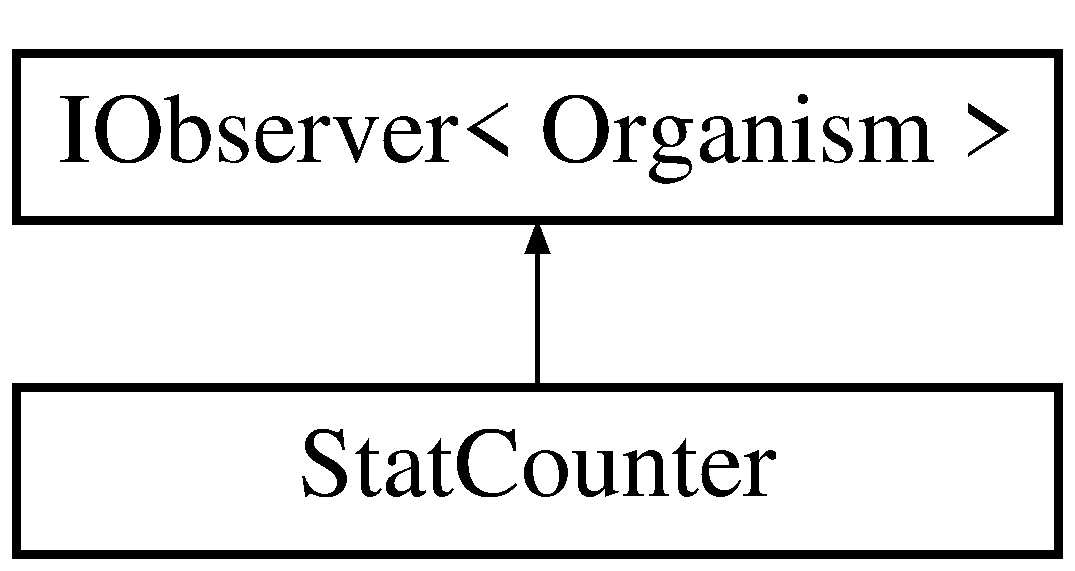
\includegraphics[height=2.000000cm]{class_stat_counter}
\end{center}
\end{figure}
\subsection*{Public Member Functions}
\begin{DoxyCompactItemize}
\item 
void \hyperlink{class_stat_counter_a81f82e98e35f1571565f2e1bc54de471}{notify} (const \hyperlink{class_organism}{Organism} \&arg) override\hypertarget{class_stat_counter_a81f82e98e35f1571565f2e1bc54de471}{}\label{class_stat_counter_a81f82e98e35f1571565f2e1bc54de471}

\begin{DoxyCompactList}\small\item\em Increments the stored counts of the genotypes and genes that arg possesses. \end{DoxyCompactList}\item 
void \hyperlink{class_stat_counter_ada1a2c28945b0bedd7840068e6cf770f}{print\+Stats} ()\hypertarget{class_stat_counter_ada1a2c28945b0bedd7840068e6cf770f}{}\label{class_stat_counter_ada1a2c28945b0bedd7840068e6cf770f}

\begin{DoxyCompactList}\small\item\em Displays the count data for genotypes and genes that have been processed. \end{DoxyCompactList}\end{DoxyCompactItemize}


\subsection{Detailed Description}
The \hyperlink{class_stat_counter}{Stat\+Counter} class records statistical data of Organisms. 

This class is meant to observe some other class that provides an implemenation of \hyperlink{class_observable}{Observable$<$\+Organism$>$}. All Organisms that are sent to \hyperlink{class_stat_counter}{Stat\+Counter} have counts of both genotypes and Genes recorded. \begin{DoxySeeAlso}{See also}
\hyperlink{struct_i_observer}{I\+Observer}, \hyperlink{class_organism}{Organism} 
\end{DoxySeeAlso}


The documentation for this class was generated from the following files\+:\begin{DoxyCompactItemize}
\item 
Genetics/Stat\+Counter.\+h\item 
Genetics/Stat\+Counter.\+cpp\end{DoxyCompactItemize}

%--- End generated contents ---

% Index
\backmatter
\newpage
\phantomsection
\clearemptydoublepage
\addcontentsline{toc}{chapter}{Index}
\printindex

\end{document}
